\documentclass{scrartcl}
\usepackage[utf8]{inputenc}
\usepackage{graphicx}
\usepackage{hyperref}
\usepackage{float}


\title{Software Engineering 2: "PowerEnJoy"\newline\newline
Requirements Analysis and\\Specification Document}
\subtitle{Version 1.0}
\author{Piccirillo Luca - 790380\\
Zampogna Gian Luca - 863097\\
Zini Edoardo - 875275}
\date{November 13, 2016}

\hypersetup{
    colorlinks,
    citecolor=black,
    filecolor=black,
    linkcolor=black,
    urlcolor=black
}

\begin{document}
\pagenumbering{gobble}
\begin{figure} [h!]
    \centering
    
\includegraphics[scale=0.6]{LogoPolimi.png}
    \label{fig:LogoPolimi}
    \maketitle
\end{figure}
\newpage
\pagenumbering{roman}
\tableofcontents
\newpage
\pagenumbering{arabic}

\section{Introduction}
\subsection{Purpose}


\subsection{Scope}


\subsection{Definitions, Acronyms, Abbreviations}
\subsubsection{Acronyms, Abbreviations}
\begin{itemize}
    \item PEJ = PowerEnJoy
    \item SBL = Service Back-end Logic: software logic of the service the user do not directly interact with.
\end{itemize}
\subsubsection{Definitions}
\begin{itemize}
\item \textbf{Car:} every vehicle, which respects the requirements, that the system allows the users to use.
    \item \textbf{Special Parking Area:} pre-defined areas (i.e. streets) where a user is allowed to park and where the batteries of the Cars can be plugged into the power grid.
    \item \textbf{Total Base Fare:} amount of money that the user pays for the ride duration only. It does not include any discount or penalty for any other specific condition.
    \item \textbf{Total Ride Fare:} amount of money that the user pays. It includes any discount or penalty for any other specific condition satisfied during the ride.
\end{itemize}

\subsection{Reference Document}
\begin{itemize}
    \item Project?s Assignment document: AA 2016-2017 Software Engineering 2 - Project goal, schedule, and rules.
    \item IEEE Std 830-1998, IEEE Recommended Practice for Software Requirements Spec- ifications.
    \item Software Engineering 2: "PowerEnJoy" Requirements Analysis and Specification Document.
    \item UX diagram PDF from the course "Sistemi Informativi" of Politecnico of Milan.
\end{itemize}

\subsection{Document Structure}
This document is split in 6 parts:
\begin{itemize}
    \item \textbf{Architectural Design:} contains the different architectural views of the system.
    \item \textbf{Algorithm Design:} contains the pseudo-codes of the most relevant algorithmic parts of the system.
    \item \textbf{User Interface Design:} contains an overview of how the user interface on the system will look like.
    \item \textbf{Requirements Traceability:} shows the correlation among the requirements defined in the RASD and the design elements contained in this document.
    \item \textbf{Effort Spent:} contains the amount of time each member spent on the document, split between time spent working together and time spent on his own.
    \item \textbf{References:} contains all the references required by this document.
\end{itemize}
\newpage
\section{Overall Description}
\subsection{Product perspective}
The PowerEnJoy service will be built by a mobile application that will let the customer search for a Car and, in case he finds a suitable ride solution, he will be guided in the process of registering to the service (if not already a PowerUser), reserving and unlocking the Car by following the instructions provided through the mobile application. The on-board infotainment will further assis the customer up to the end of his ride. Customers will only need to interact with those two system elements to access and make use of the service.
\subsubsection{Quality of Service}
%TODO è simile ai CONTRAINTS che ci sono poco più avanti
\begin{itemize}
    \item \textbf{Availability:} the system must be available during the diurnal hours, manitenace should be perfomed only during the night when the number of requests is lower.
    %AVAILABILITY: % of time the system is available to the users.
     %TODO non mi vengono molte idee, dite di lasciare questa voce? Non mi piace molto
    \item \textbf{Exceptions Handling:} the system must be able to handle exceptions in case of unsatisfying domain properties e.g. Credit card without enough money,...
    %TODO it's the same of CONSTRAINTS, this make no sense considering the availability request
    \item \textbf{Reliability:} the system does not have any reliability requirements.
    %RELIABILITY: time the service runs without interruptions.
      \item \textbf{Scalability:} the system must be able to properly manage an increasing number of users, or an unexpected peak of the number of request.
    \item \textbf{Security:} the system must protect user data and ensure that online secure connections take place among the service, the user and the payment structure the system relies on.
    \item \textbf{Usability:} the interface will be user-friendly (i.e. it will always shows the user only the actions he can actually perform) and will not use a red-green color combination in order to always be clear for all users, including the color blind ones.
    %TODO cosa ne pensate???
\end{itemize}
\subsection{Product functions}
For better orienteering through this document, here is a main functionality summary.
\begin{itemize}
\item Car's map explorer
\item Personal account management
\item Car reservation assistant
\item On-board ride assistant
\item Automatic payment processing
\item Remote vehicle interfacing
\end{itemize}
\subsection{User characteristics}
All kinds of user interaction with the system start from the mobile application or the onboard car's infotainment equipment. A Visitor can only have a preview of service availability just by opening up the application. All other functionalities will require the user to authenticate against the service as a PowerUser.
\subsection{Constraints}
\subsubsection{Regulatory policies}
The system must satisfy existing privacy regulations about user's sensible data.
\subsubsection{Interfaces to other applications}
The system must be compatible with payment API provided by the existing financial services partner.
\subsubsection{Parallel operation}
Management software components must support simultaneous multi-customer operations 
\subsubsection{Reliability requirements}
PoweEnJoy does not ask for any reliability requirements.
\subsubsection{Criticality of the application}
The mobile application is the only customer entry point to the service. Any malfunction in the mobile application will actually prevent a customer from accessing the service.
\subsubsection{Safety and security considerations}
The system must not disclose customers private service-related information without the appropriate permissions.
\subsection{Assumptions and dependencies}
\begin{itemize}
\item Cars belonging to PowerEnJoy have a clearly recognizable logo.
\item Cars are already equipped with onboard infotainment device which is able to provide basic offline navigation services in case of missing Internet connectivity.
\item All Cars have an interface that is able to provide any kind of data from all sensors available in the car itself.
\item Availability of the following sensors (or functional equivalents) is assumed: GPS receiver, battery status, core vehicle diagnostics.
\item Onboard navigation software will not be developed, an existing solution will be integrated.
\item Predefined Safe Areas are assumed to be under mobile data connectivity service coverage.
\item Special Parking Areas and exclusive power sockets allocation are pre-determined in such a way that spreading Cars among all the available sockets and filling them all corresponds to the best possible distribution of vehicles.
\item The end-user device used to access the service by the mobile app are able to send geolocation data while nearby the booked Car (ie. both data connectivity and GPS sensors are functional).
\end{itemize}
\subsection{Goal Summary}
\begin{enumerate}[label={[}G\arabic*{]}]
\item Allow any kind of user to view the map of the available nearby Cars.
\item Allow Visitor user to register to the service.
\item Allow Visitor user to log-in and out as a PowerUser.
\item Allow PowerUser to check the status of the Car.
\item Allow PowerUser to reserve a Car.
\item Allow PowerUser to cancel a reservation.
\item Allow PowerUser to check the position of the reserved car.
\item Allow PowerUser to unlock and enter the Car when inside the specific range.
\item Allow PowerUser to get driving directions to his destination.
\item Allow PowerUser to see a list of the closest Special Parking Areas to his destination.
\item Allow PowerUser to keep track of the current charge. 
\item Allow PowerUser to know whether he can be eligible for any discount or penalty.
\item Allow the PowerUser to get a money saving alternative destination.
\item Allow the system to lock the Car in a Safe Parking Area at the end of the ride.
\item Allow the system to apply penalty or discount according to the given criteria.
% Are PARAMETRIC CRITERIA reasonable??
\item Let the system bill the PowerUser for the total ride price and issue a payment request for that amount at the end of the ride.
%TODO
\item GOAL ADMINISTRATION ACCESS
\end{enumerate}
\newpage
\section{Scenarios}

\subsection{Scenario 1: Typical usage situation}
Al is a student and he have to go to University, however public transport is on strike, so he decides to rent a Car.  He installs the PowerEnJoy app on his mobile phone, he opens it and looks for a nearby Car on the map. He find one at 200 meters from his home. At this point he decides to register to the PEJ service fulfilling all camps with his name, surname, driver licence, email and credit card information. He receives the mail with the password, he logs in as PowerUser, and he reserves the previously seen Car. In 20 minutes he is near the car. He opens the app to confirm his proximity to the Car, the system let him ask the unlocking of the Car so that Al can enter, insert his destination on the screen of the Car, start the engine and drive towards his destination. During the ride he can keep the current battery level and the charge under control watching them on Car screen. Once arrived he stops, parks and since he read on the Car screen that he is inside a Safe Parking Area he exits and leaves the Car. The Car is locked automatically after one minute and the total charge is deducted from his payment method. Al receives a mail containing the details about the duration and the discount of his ride.

\subsection{Scenario 2: No Car available}
John has just left a party, his only wish is to get home as soon as possible but unfortunately he finds out that his car does not start. Looking around he sees a Car with the PowerEnJoy logo on the side. He googles it and find a way to install the PowerEnJoy app. After opening it, he starts looking for that Car in order to reserve it, however he discovers that it is not shown on the map, so it can't be rented. At that point he gives up and falls back to the night service of the local public transport.

\subsection{Scenario 3: Car pooling discount}
Jack is an architect, and he is expected to attend a meeting located in the other side of the city. The day before he finds out that due to the high pollution level his old car is not authorized to be used. Since he needs to carry a lot of big papers with him, he does not want to use the public transport. He decided to rent a car using the PowerEnJoy service. Furthermore he proposes to a neighbour to share the ride, so since both Jack, his wife and his neighbour need to reach the same destination, they are eligible for a discount. The following day Jack launches the PowerEnJoy app, selects the closest Car and, with both his wife and his neighbour, reaches his destination and parks. They leave the Car, and since there were at least three people from the beginning of the journey up to the end, the system applies a discount before deducting the charge. Jack receives a mail confirming the final charged with the discount already applied.

\subsection{Scenario 4: Charged ($\geq$50\%) battery discount}
Elizabeth is attending the local gym, she doesn't live too far from it, but she is not comfortable walking alone in the evening. So she decides to take advantage of the PowerEnJoy service, since there is a Special Parking Area few meters from her home. Once arrived to the gym and stopped the Car, she finds out that she has consumed far less than half of the battery. Since she is eligible for a discount the system applied it before deducting the charge.

\subsection{Scenario 5: Money saving option}
Victor is an hard worker, he has just moved from another city and he hasn't bought a car yet since he need to save as much money as possible. He has just discovered the existence of the PowerEnJoy service and its money saving option. He downloads the app, launches it, completes the registration and reserves a near Car. Jack gets in the Car before his reservation expires and inserts his destination on the screen of the Car. He enables the money saving option and the navigator shows the Special Parking Areas where he have to park to get a discount. Jack considers that solution suitable for his needs, so he starts his ride. The navigator drives him to the Special Parking Area, John parks the Car and exits it. Within the prescribed time limit he plugs the Car into the power grid, this way the discount is applied.

\subsection{Scenario 6: Reservation cancelled}
Elena is working as babysitter looking after the son of her friends. She only left her friends' house when the child's parents are back, and since they are very punctual people she has already reserved a Car using the PoweEnJoy app. Unfortunately, due to a traffic jam, they are late; after they informed her she opens the PowerEnjoy app and cancels her reservation.

\subsection{Scenario 7: 1$\euro$ fee}
Nathan and Samuel are two brothers. They reserved a Car in order to go to the cinema. They are leaving home when a water pipe breaks and starts pouring water everywhere in the kitchen. They immediately close the water, but since there is water everywhere they decide to stay home and clean up the wet floor. They forget their reservation, so after the established hour the system deducts the 1$\euro$ penalty and sends an email to Nathan, who is the PowerUser, noticing him about it.
\newpage
\section{Specific Requirements}
Text
\subsection{External interface requirements}
Text
\subsubsection{User interfaces}


\begin{figure}[h!]
    \centering
    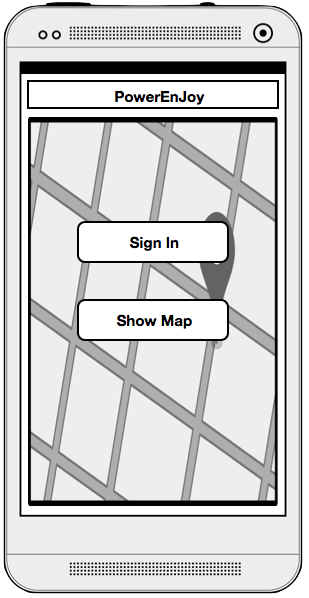
\includegraphics[scale=0.3]{{Figures/Mockup/1FirstScreen.png}}
    \label{fig:1FirstScreen}
    \\From the first screen a user can either sign in, or create a new account if he is a new user, or consult the map of available Cars.
\end{figure}

\begin{figure}[h!]
    \centering
    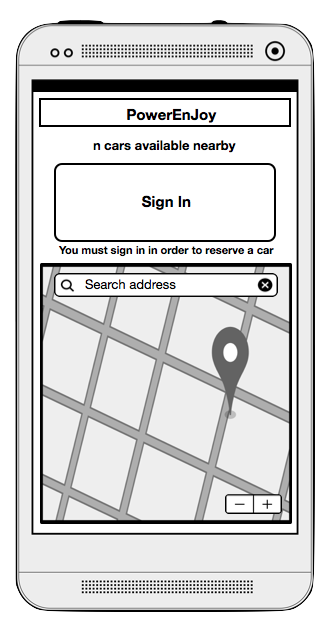
\includegraphics[scale=0.3]{{Figures/Mockup/2MapNotLogged.png}}
    \label{fig:2MapNotLogged}
    \\If a user chooses the map, he will see a map with all the available cars and he will be asked to sign in in order to proceed with the reservation.
\end{figure}


\begin{figure}[p!]
    \centering
    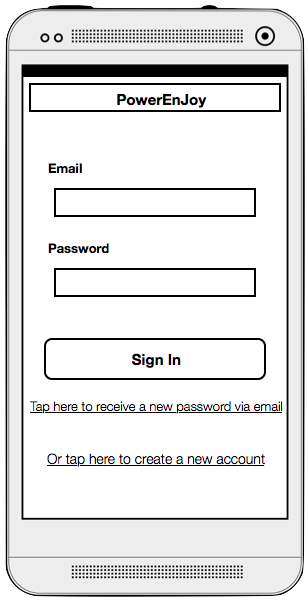
\includegraphics[scale=0.3]{{Figures/Mockup/3LoginForm.png}}
    \label{fig:3LoginForm}
    \\Whether a user started from the map or from the first screen, he will have to either enter his credential or register. In case of forgotten credential he is given the possibility to ask for a new password too.
\end{figure}

\begin{figure}[p!]
    \centering
    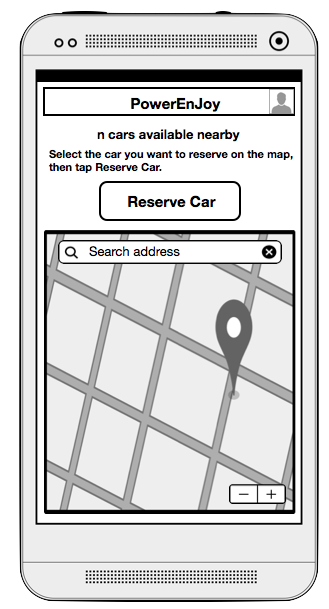
\includegraphics[scale=0.3]{{Figures/Mockup/4CarReservationA}}
    \label{fig:4CarReservationA}
    \\A PowerUser can look for a suitable Car nearby his position, or entering an adress in the appropriate bar above the map. After finding a Car the PowerUser can reserve it.
\end{figure}

\begin{figure}[p!]
    \centering
    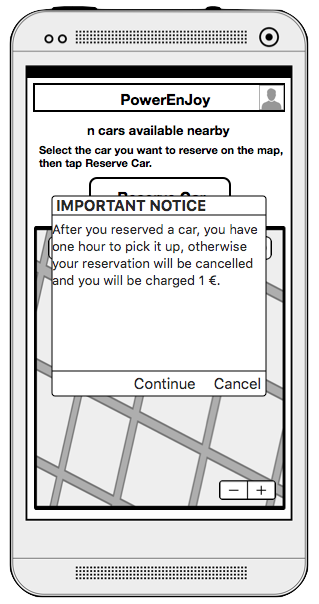
\includegraphics[scale=0.3]{{Figures/Mockup/4CarReservationB.png}}
    \label{fig:4CarReservationB}
    \\Before actually reserving a Car, the system reminds the PowerUser about the one hour expiration of his reservation and the relative penalty fee.
\end{figure}

\begin{figure}[p!]
    \centering
    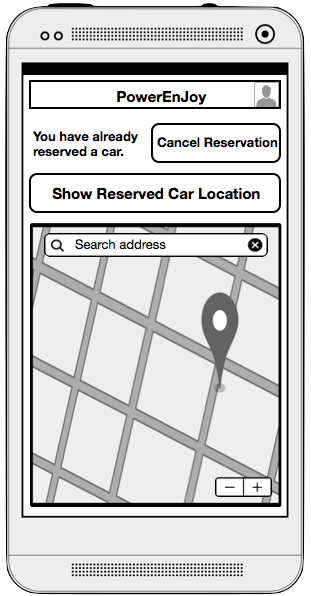
\includegraphics[scale=0.3]{{Figures/Mockup/5CarReserved.png}}
    \label{fig:5CarReserved}
    \\The selected Car has been reserved. Now a PowerUser can cancel his reservation or look for his car thanks to the provided map.
\end{figure}

\begin{figure}[p!]
    \centering
    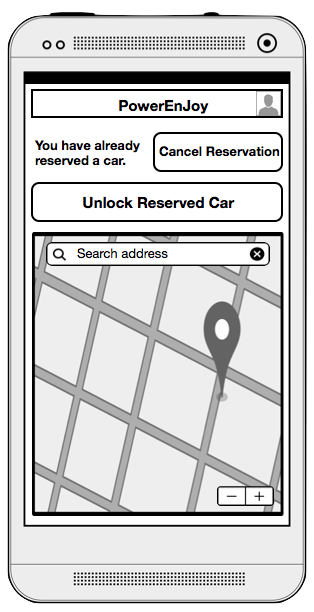
\includegraphics[scale=0.3]{{Figures/Mockup/6CarNearby.png}}
    \label{fig:6CarNearby}
    \\When a PowerUser is near his reserved Car, he is given the possibility to ask the system to unlock it. If the PowerUser changes his mind he can still cancel the reservation, this possibility will remain valid until the PowerUser ignites the engine. 
\end{figure}

\begin{figure}[p!]
    \centering
    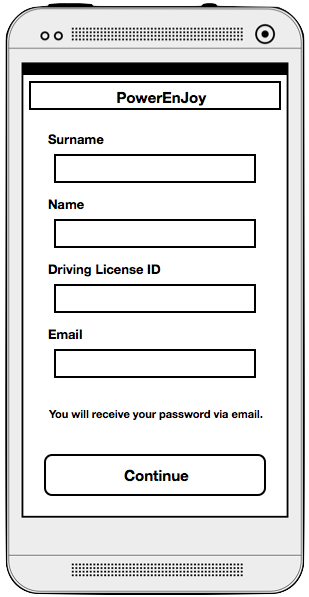
\includegraphics[scale=0.3]{{Figures/Mockup/7RegistrationFormA.png}}
    \label{fig:7RegistrationFormAForm}
    \\This is the first page that requires a new user to enter his personal data.
\end{figure}

\begin{figure}[p!]
    \centering
    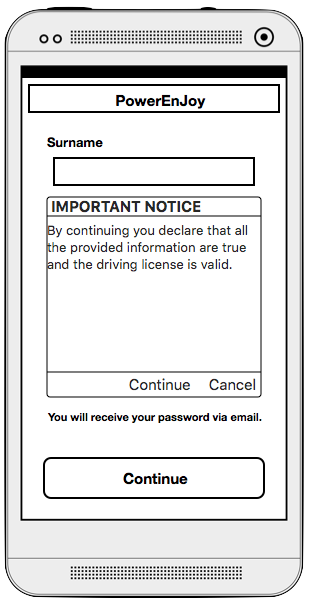
\includegraphics[scale=0.3]{{Figures/Mockup/7RegistrationFormB.png}}
    \label{fig:7RegistrationFormB}
    \\In order to stress the importance for the user to enter real and correct data, the system reminds the user about this.
\end{figure}

\begin{figure}[p!]
    \centering
    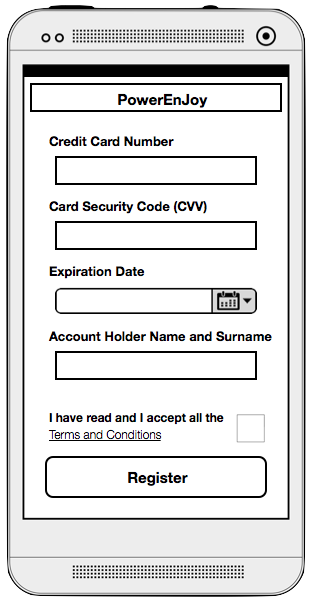
\includegraphics[scale=0.3]{{Figures/Mockup/7RegistrationFormC.png}}
    \label{fig:7RegistrationFormCnForm}
    \\Last page of the registration form, the user is asked for his payment information. Furthermore he will have to accept the terms and conditions of the service in order to complete the registration.
\end{figure}

\begin{figure}[p!]
    \centering
    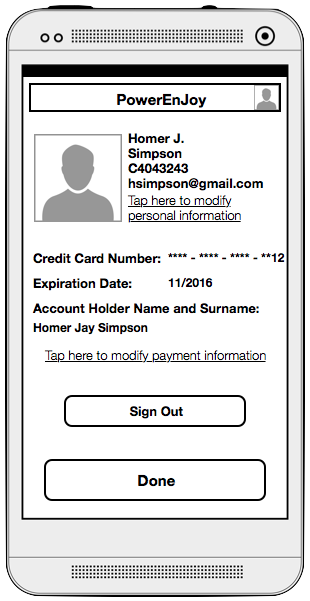
\includegraphics[scale=0.3]{{Figures/Mockup/8PersonalAccountPage.png}}
    \label{fig:8PersonalAccountPage}
    \\A PowerUser can access his personal account page by tapping on the avatar in the up right corner of his screen. By doing so, this is what he will be shown. From this page it is also possible to modify both personal and payment information.
\end{figure}

\begin{figure}[p!]
    \centering
    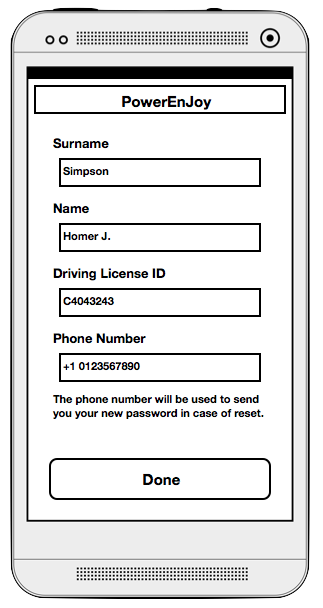
\includegraphics[scale=0.3]{{Figures/Mockup/9PersonalDataModification.png}}
    \label{fig:9PersonalDataModification}
    \\This is the page to be used by a PowerUser in order to modify his personal information.
\end{figure}

\begin{figure}[h!]
    \centering
    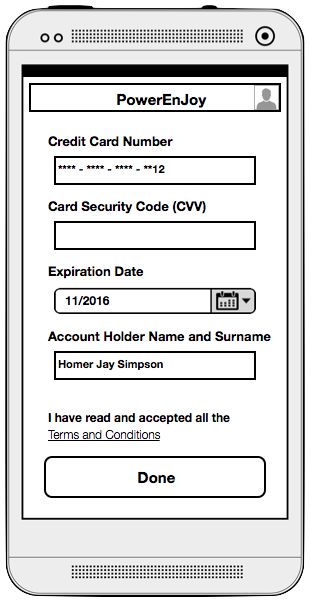
\includegraphics[scale=0.3]{{Figures/Mockup/10PaymentSystemDataModification.png}}
    \label{fig:10PaymentSystemDataModificationForm}
    \\This is the page to be used by a PowerUser in order to modify his payment information.
\end{figure}

\subsubsection{Hardware interfaces}
Text
\subsubsection{Communication interfaces}
Text
\subsubsection{Software interfaces}
Text
\subsection{Functional requirements}

\newcounter{goalctr}
    \stepcounter{goalctr}
    \subsubsection{Goal \arabic{goalctr}}
    {[}G\arabic{goalctr}{]}
    Allow any kind of user to view the map of the available nearby Cars
    \begin{itemize}
        \item Requirements
        \begin{enumerate}[label={[}R\arabic*{]},series=REQ]
    		\item Users must have access to a map indicating the user current location.
    		\item Users must be able to pan and scroll the map in any direction.
    		\item Every available Car must be shown on a map.
        \end{enumerate}
        \item Domain properties
        \begin{enumerate}[label={[}P\arabic*{]},series=PRO]
    			\item No Car with less than B\% battery charge is taken into account as available for booking.
    			\item No Car that is currently under charging and has less than C\% battery charge is taken into account as available for booking.
        \end{enumerate}
    \end{itemize}
    
    \stepcounter{goalctr}
    \subsubsection{Goal \arabic{goalctr}}
    {[}G\arabic{goalctr}{]}
    Allow Visitor user to register to the service.
    \begin{itemize}
        \item Requirements
        \begin{enumerate}[REQ]
    		\item Let a Visitor user start the registration wizard while he's still not logged in.
			\item The registration form must contain input fields for user identity, email, contact info, driving license number and expiration, privacy agreement confirmation, customer notifications and subscriptions options, credit card number and expiration, billing identity.
			\item The chosen email address must not be already used by another PowerUser.
			\item The credit card must be verified not to be blocked or expired upon registration.
			\item The user must receive a system generated password to the registered email address.
        \end{enumerate}
        \item Domain properties
        \begin{enumerate}[PRO]
    			\item None
        \end{enumerate}
    \end{itemize}

    \stepcounter{goalctr}
    \subsubsection{Goal \arabic{goalctr}}
    {[}G\arabic{goalctr}{]}
    Allow Visitor user to log-in and out as a PowerUser.
    \begin{itemize}
        \item Requirements
        \begin{enumerate}[REQ]
			\item A Visitor user must always see an input to access log-in form as long as he's still not logged in.
		    \item An input to perform log-out must always be available to the PowerUser if he's currently logged in.
        \end{enumerate}
        \item Domain properties
        \begin{enumerate}[PRO]
    			\item None
        \end{enumerate}
    \end{itemize}

    \stepcounter{goalctr}
    \subsubsection{Goal \arabic{goalctr}}
    {[}G\arabic{goalctr}{]}
    Allow PowerUser to check the status of the Car.
    \begin{itemize}
        \item Requirements
        \\For each Car shown to the PowerUser, he must be able to access information regarding:
        \begin{enumerate}[REQ]
    		\item remaining battery charge
			\item current position
        \end{enumerate}
        \item Domain properties
        \begin{enumerate}[PRO]
    			\item None
        \end{enumerate}
    \end{itemize}

    \stepcounter{goalctr}
    \subsubsection{Goal \arabic{goalctr}}
    {[}G\arabic{goalctr}{]}
    Allow PowerUser to reserve a Car.
    \begin{itemize}
        \item Requirements
        \begin{enumerate}[REQ]
    		\item The PowerUser must have the ability to start the reservation wizard for any available Car.
			\item The PowerUser must see a reminder about unfulfilled reservation penalty before confirmation.
			\item Show an input to allow the PowerUser to confirm and finalize the reservation.
        \end{enumerate}
        \item Domain properties
        \begin{enumerate}[PRO]
    			\item None
        \end{enumerate}
    \end{itemize}

    \stepcounter{goalctr}
    \subsubsection{Goal \arabic{goalctr}}
    {[}G\arabic{goalctr}{]}
	Allow PowerUser to check the position of the reserved car.
    \begin{itemize}
        \item Requirements
        \begin{enumerate}[REQ]
    	    \item As long as a reservation exists for the PowerUser an input must be available to give him the position of that Car on the map.
        \end{enumerate}
        \item Domain properties
        \begin{enumerate}[PRO]
    		\item None
        \end{enumerate}
    \end{itemize}

    \stepcounter{goalctr}
    \subsubsection{Goal \arabic{goalctr}}
    {[}G\arabic{goalctr}{]}
	Allow PowerUser to unlock and enter the Car when inside the specific range.
    \begin{itemize}
        \item Requirements
        \begin{enumerate}[REQ]
    	    \item The system must be able to remotely unlock the Car.
			\item The system must be able to compute the distance between the user location and his reserved Car.
			\item Show an input to the PowerUser allowing to send an unlock request.
        \end{enumerate}
        \item Domain properties
        \begin{enumerate}[PRO]
    			\item None
        \end{enumerate}
    \end{itemize}
    
    \stepcounter{goalctr}
    \subsubsection{Goal \arabic{goalctr}}
    {[}G\arabic{goalctr}{]}
    Allow PowerUser to get driving directions to his destination.
    \begin{itemize}
        \item Requirements
        \begin{enumerate}[REQ]
    			\item The user must be allowed to select a custom destination and start navigating to that location.
        \end{enumerate}
        \item Domain properties
        \begin{enumerate}[PRO]
    			\item Navigation software always provides effective directions to the user if destination it's included in Safe Areas.
        \end{enumerate}
    \end{itemize}

    \stepcounter{goalctr}
    \subsubsection{Goal \arabic{goalctr}}
    {[}G\arabic{goalctr}{]}
    Allow PowerUser to see a list of the closest Special Parking Areas to his destination.
    \begin{itemize}
        \item Requirements
        \begin{enumerate}[REQ]
    		\item The system must capable of providing a list of Special Parking Areas sorted by distance from an input location.
			\item PowerUser must be allowed anytime during the navigation to input a custom location and be acknowledged about all nearest Special Parking Areas from the selected location.
        \end{enumerate}
        \item Domain properties
        \begin{enumerate}[PRO]
    			\item None
        \end{enumerate}
    \end{itemize}
    
    \stepcounter{goalctr}
    \subsubsection{Goal \arabic{goalctr}}
    {[}G\arabic{goalctr}{]}
    Allow PowerUser to keep track of the current charge.
    \begin{itemize}
        \item Requirements
        \begin{enumerate}[REQ]
    			\item None
        \end{enumerate}
        \item Domain properties
        \begin{enumerate}[PRO]
    			\item None
        \end{enumerate}
    \end{itemize}
    
    \stepcounter{goalctr}
    \subsubsection{Goal \arabic{goalctr}}
    {[}G\arabic{goalctr}{]}
    Allow PowerUser to check whether he can be eligible for any discount or penalty.
    \begin{itemize}
        \item Requirements
        \begin{enumerate}[REQ]
    			\item None
        \end{enumerate}
        \item Domain properties
        \begin{enumerate}[PRO]
    			\item None
        \end{enumerate}
    \end{itemize}
    
    \stepcounter{goalctr}
    \subsubsection{Goal \arabic{goalctr}}
    {[}G\arabic{goalctr}{]}
    Notify the PowerUser of the total amount of charged money via Car screen.
    \begin{itemize}
        \item Requirements
        \begin{enumerate}[REQ]
    			\item None
        \end{enumerate}
        \item Domain properties
        \begin{enumerate}[PRO]
    			\item None
        \end{enumerate}
    \end{itemize}
 
    \stepcounter{goalctr}
    \subsubsection{Goal \arabic{goalctr}}
    {[}G\arabic{goalctr}{]}
    Allow PowerUser to cancel a reservation.
    \begin{itemize}
        \item Requirements
        \begin{enumerate}[REQ]
    			\item None
        \end{enumerate}
        \item Domain properties
        \begin{enumerate}[PRO]
    			\item None
        \end{enumerate}
    \end{itemize}
 
    \stepcounter{goalctr}
    \subsubsection{Goal \arabic{goalctr}}
    {[}G\arabic{goalctr}{]}
    Allow the PowerUser to get a money saving alternative destination.
    \begin{itemize}
        \item Requirements
        \begin{enumerate}[REQ]
    			\item None
        \end{enumerate}
        \item Domain properties
        \begin{enumerate}[PRO]
    			\item Special Parking Areas provide at least N\# power sockets as exclusively available to PowerEnJoy customers.
        \end{enumerate}
    \end{itemize}
 
    \stepcounter{goalctr}
    \subsubsection{Goal \arabic{goalctr}}
    {[}G\arabic{goalctr}{]}
    Allow the system to calculate the total billing amount at the end of the ride.
    \begin{itemize}
        \item Requirements
        \begin{enumerate}[REQ]
    			\item None
        \end{enumerate}
        \item Domain properties
        \begin{enumerate}[PRO]
    			\item None
        \end{enumerate}
    \end{itemize}
 
    \stepcounter{goalctr}
    \subsubsection{Goal \arabic{goalctr}}
    {[}G\arabic{goalctr}{]}
    Allow the system to apply penalty or discount according to the given criteria.
    \begin{itemize}
        \item Requirements
        \begin{enumerate}[REQ]
    			\item None
        \end{enumerate}
        \item Domain properties
        \begin{enumerate}[PRO]
    			\item None
        \end{enumerate}
    \end{itemize}
 
    \stepcounter{goalctr}
    \subsubsection{Goal \arabic{goalctr}}
    {[}G\arabic{goalctr}{]}
    Allow the system to lock the Car in a Safe Parking Area at the end of the ride.
    \begin{itemize}
        \item Requirements
        \begin{enumerate}[REQ]
    			\item None
        \end{enumerate}
        \item Domain properties
        \begin{enumerate}[PRO]
    			\item At least a free parking slot is available for the user among all Safe Areas.
        \end{enumerate}
    \end{itemize}

\subsection{Use cases}
Text
\newpage
\section{Appendix}

\subsection{References}
\begin{itemize}
    \item \url{https://cwiki.apache.org/confluence/display/OFBIZ/Multitenancy+support}
    \item \url{https://cwiki.apache.org/confluence/display/OFBADMIN/Mini+Language+-+minilang+-+simple-method+-+Reference}
\end{itemize}

\subsection{Effort Spent}
\begin{tabular}{| p{5cm} | p{5cm} |}
\hline
Teamwork & $\sim$4h\\
\hline
Piccirillo Luca & $\sim$5h\\
\hline
Zampogna Gian Luca & $\sim$8h\\
\hline
Zini Edoardo & $\sim$5h\\
\hline
\end{tabular}


\subsection{Revision History}
\begin{tabular}{| l | l | p{10cm} |}
\hline
\textbf{Version} & \textbf{Date} & \textbf{Changes}\\
\hline
1.0-RC1 & 05/02/2017 & First deadline release.\\
\hline
\end{tabular}

\end{document}